\subsection{Basic Terminology and Techniques}

% An example of joint probability function table...
% \[
%     \begin{array}{cc|ccc|c}
%         & & \multicolumn{3}{c|}{x} & \\
%         \multicolumn{2}{c|}{f(x,y)} & 0 & 1 & 2 & \\
%         \hline
%         y & 1 & 0.1 & 0.2 & 0.3 & \\
%           & 2 & 0.2 & 0.1 & 0.1 & \\
%         \hline
%         & & & & & 1
%     \end{array}
% \]



\begin{definition}[\textbf{Joint Probability Function}]
    \phantom{}\\
    Let $X$ and $Y$ be two discrete random variables, we define the \textbf{joint probability function}
    $f(x, y)$ of $(X, Y)$ as \vspace{-3mm}
    \begin{align*}
        f(x, y) &= P(X = x \; \text{and} \; Y = y)    \\
                &= P(X = x, Y = y)
    \end{align*}
\end{definition}

\begin{remark}
    In general, if there are $n$ discrete random variables $X_1, X_2, \ldots, X_n$, we have \vspace{-2mm}
    \[f(x_1, x_2, \ldots, x_n) = P(X_1 = x_1, X_2 = x_2, \ldots, X_n = x_n).\]
\end{remark}


\begin{theorem}[\textbf{Properties of Joint Probability Function}]
    \phantom{}\
    \begin{itemize}
        \item $f(x, y) > 0 \; \forall (x, y)$.
        \item $\dis \sum_{\text{all } (x, y)} f(x, y) = 1$.
    \end{itemize}
\end{theorem}


\begin{example}
    Let $X$ be the number of daily purchases of a luxury item from a factory outlet location and Y be the daily number of purchases made online. Let 1,2, and 3 denote the number of purchases less than five, at least five but less than 15, and 15 or more respectively. The joint pf of X and Y is
    \[
        \begin{array}{cc|ccc|c}
            & & \multicolumn{3}{c|}{x} & \\
            \multicolumn{2}{c|}{f(x,y)} & 1 & 2 & 3 & \\
            \hline
            \multirow{3}{*}{y} 
              & 1 & 0.09 & 0.12 & 0.13 & \\
              & 2 & 0.12 & 0.11 & 0.11 & \\
              & 3 & 0.13 & 0.10 & 0.09 & \\
            \hline
            & & & & & 1
        \end{array}
    \]

    Find $f(1,2)$ and $f(2,2)$.

    \textbf{Solution:} $f(1,2) = P(X=1, Y=2) = 0.12$ and $f(2,2) = P(X=2, Y=2) = 0.11$.
\end{example}

\pagebreak

\textbf{What if we are only interested in \underline{one} of the variables?}

\begin{example}[continued]
    Say, we are only interested in $X$. Then, \vspace{-3mm}
    \begin{align*}
        P(X = 1) = P(B) &= P(B \cap A_1) + P(B \cap A_2) + P(B \cap A_3) \\
        & = P(X=1,Y=1) + P(X=1,Y=2) + P(X=1,Y=3) \\
        & = 0.34.
    \end{align*}
    Similarly, $P(X=2) = 0.33$ and $P(X = 3) = 0.33$.
\end{example}

\begin{note}
    \phantom{}\
    \begin{itemize}
        \item $\displaystyle \sum_{\text{all } x} f_X(x) = \displaystyle \sum_{\text{all } y} f_Y(x) = \displaystyle \sum_{\text{all } (x,y)} f_{X,Y}(x,y) = 1$.
    \end{itemize}
\end{note}


\begin{definition}[\textbf{Marginal Distributions}]
    \phantom{}\\
    Given the joint probability function of $X$ and $Y$, the \textbf{Marginal distributions} are give by
    \begin{itemize}
        \item $f_1(x) = f_X(x) = \displaystyle \sum_{\text{all } y} f_X(x)$, with $x$ fixed.
        \item  $f_2(y) = f_Y(y) = \displaystyle \sum_{\text{all } x} f_X(x)$, with $y$ fixed.
    \end{itemize}
\end{definition}

\begin{remark}
    This idea can be extended beyond two variables.
\end{remark}

\begin{definition}[\textbf{Independent Random Variables}]
    \phantom{}\\
    $X$ and $Y$ are \textbf{independent} random variables $\iff$ $f(x, y) = f_1(x)f_2(y)$,
    $\forall$ $(x, y)$.
\end{definition}

In general, $X_1, X_2, \ldots, X_n$ are independent variables \vspace{-3mm}
    \[\iff f(x_1, x_2, \ldots, x_n) = f_1(x_1)f_2(x_2) \cdots f_n(x_n) \quad \forall x_1, x_2, \ldots, x_n.\]

\begin{remark}
    You can only conclude that $X$ and $Y$ are independent after checking \underline{ALL} $(x,y)$ combinations.
\end{remark}

\pagebreak

\begin{definition}[\textbf{Conditional Probability Function}]
    \phantom{}  \\
    The conditional probability function of $X$ given $Y = y$ is
    \[f_1(x|y) = \frac{f(x, y)}{f_2(y)} \quad \text{provided $f_2(y) > 0$}.\]
    Similarly, the conditional probability function of $Y$ given $X = x$ is
    \[f_2(y|x) = \frac{f(x, y)}{f_1(x)} \quad \text{provided $f_1(x) > 0$}.\]
\end{definition}

\begin{note}
    \phantom{}
    \begin{itemize}
        \item $f_1(x) = f_X(x)$ and $f_2(y) = f_Y(y)$.
        \item $\displaystyle \sum_{\text{all } x} f(x|y) = 1$.
    \end{itemize}
\end{note}

\begin{example}
    Continuing with our example:
    \[
        \begin{array}{cc|ccc|c}
            & & \multicolumn{3}{c|}{x} & \\
            \multicolumn{2}{c|}{f(x,y)} & 1 & 2 & 3 & f_Y(y) \\
            \hline
            \multirow{3}{*}{y} 
              & 1 & 0.09 & 0.12 & 0.13 & 0.34 \\
              & 2 & 0.12 & 0.11 & 0.11 & 0.34 \\
              & 3 & 0.13 & 0.10 & 0.09 & 0.32 \\
            \hline
            \multicolumn{2}{c|}{f_X(x)} & 0.34 & 0.33 & 0.33 & 1
        \end{array}
    \]
    Find the conditional probability function of $X$ given $Y = 1$, i.e find $f(x|1)$.

    \textbf{Solution:} Since $f(x|1) = \frac{f(x,1)}{f_Y(1)}$, we have \vspace{-2mm}
    \[
        \begin{array}{c|ccc|c}
            x & 1 & 2 & 3 & \text{Total} \\
            \hline
            f(x|1) & \frac{0.09}{0.34} = 0.26 & \frac{0.12}{0.34} = 0.35 & \frac{0.13}{0.34} = 0.38 & 1 \\
        \end{array}
    \]  
\end{example}

\begin{remark}
    If $X$ and $Y$ are independent, then $f(x|y) = \frac{f_1(x) f_2(y)}{f_2(y)} = f_1(x)$.
\end{remark}

\pagebreak

\textbf{Functions of Random Variables}

\begin{example}
    Let $U = Y - X$, where $X$ and $Y$ have the joint probability function given below. We might now be interested in finding the probability function of $U$, which is a function of $X$ and $Y$.
    \[
        \begin{array}{cc|ccc|c}
            & & \multicolumn{3}{c|}{x} & \\
            \multicolumn{2}{c|}{f(x,y)} & 1 & 2 & 3 & f_Y(y) \\
            \hline
            \multirow{3}{*}{y} 
              & 1 & 0.09 & 0.12 & 0.13 & 0.34 \\
              & 2 & 0.12 & 0.11 & 0.11 & 0.34 \\
              & 3 & 0.13 & 0.10 & 0.09 & 0.32 \\
            \hline
            \multicolumn{2}{c|}{f_X(x)} & 0.34 & 0.33 & 0.33 & 1
        \end{array}
    \]
    The possible values of $U$ are seen by looking at the value of $u = y - x$ for each $(x,y)$ in the range of $(X,Y)$.
    \[
        \begin{array}{cc|ccc}
            & & \multicolumn{3}{c}{x}  \\
            \multicolumn{2}{c|}{u}
            & 1 & 2 & 3 \\
            \hline
            \multirow{3}{*}{y}
            & 1 & 0 & -1 & -2 \\
            & 2 & 1 & 0 & -1 \\
            & 3 & 2 & 1 & 0
        \end{array}
    \]
    $P(U = 0) = P(X=1,Y=1) + P(X=2,Y=2) + P(X=3,Y=3) = 0.09 + 0.11 + 0.09 = 0.29$. Similarly for other values of $U$.
\end{example}

Let $T = X + Y$. Notice that to find $P(T=t)$, we are simply adding the probabilities for all $(x,y)$ combinations such that $x + y = t$. This could be written as:
\[
    f_T(t) = P(T=t) = \sum_{\substack{\text{all } (x, y) \\ \text{with } x + y = t}} f(x,y).
\]
However, if $x+y = t$, then $y = t - x$, so we have:
\[
    f_T(t) = P(T=t) = \sum_{\substack{\text{all } x}} f(x,y) = \sum_{\substack{\text{all } x}} P(X=x,Y=t-x).
\]

\pagebreak


In general, to find the probability function for $U = g(X,Y)$ of two random variables $X$ and $Y$, we have
\[
    f_U(u) = P(U = u) = \sum_{\substack{\text{all } (x, y) \\ \text{with } g(x,y)=u}} f(x,y).
\]

This can also be extended to functions beyond two random variables. \\

\begin{theorem}
    \phantom{}\\
    If $X \sim \text{Poisson}(\mu_1)$ and $Y \sim \text{Poisson}(\mu_2)$ are independent, then 
    $T = X + Y \sim \text{Poisson}(\mu_1 + \mu_2)$.
\end{theorem}


\begin{theorem}
    \phantom{}\\
    If $X \sim \text{Binomial}(n, p)$ and $Y \sim \text{Binomial}(m, p)$ are independent, then \\
    $T = X + Y \sim \text{Binomial}(n + m, p)$.
\end{theorem}
\phantom{}

\begin{example}
    In an auto parts company, an average of $\mu$ defective parts are produced per shift. The number, $X$, of defective parts produced has a Poisson distribution.
    An inspector checks all parts prior to shipping them, but there is a 10\% chance that a defective part will slip by undetected.

    Let $Y$ be the number of defective parts the inspector finds on a shift. Find $f(x|y)$.

    i.e. The company wants to know how many defective parts are produced, but can only know the number which are actually detected.

    \textbf{Solution:} The author was also studying for Actsc 231, so did not have enough time to bother writing out the entire solution. But here is the answer:
    \[
        f(x|y) = \frac{e^{-\mu (1-p)} (\mu (1-p))^{x-y}}{(x-y)!} \quad \text{for x = y, y+1, \ldots}
    \]
\end{example}

\pagebreak

\subsection{Mutinomial Distribution}

This is a generalization of the Binomial to the case where each trial has $k$ possible outcomes.

\textbf{Physical Setup:} Similar to Binomial, except that now we have $\mathbf{k}$ types of outcomes. The experiment is repeated \textbf{independently} $\mathbf{n}$ times whith $\mathbf{k}$ \textbf{distinct outcomes} each time.

Let the probabilities of these $\mathbf{k}$ types be $\mathbf{p_1,p_2,\ldots,p_k}$ each time. Let $\mathbf{X_1} = \#$ of times the $1^{\text{st}}$ type occurs, \dots \, , $\mathbf{X_k} = \#$ of times the $k^{th}$ type occurs. Then $\left( X_1,X_2,\ldots,X_k \right)$ has a Multinomial distribution.

\begin{note}
    \phantom{}
    \begin{enumerate}
        \item $p_1 + p_2 + \cdots + p_k = 1$.
        \item $X_1 + X_2 + \cdots + X_k = n$. \\
        If we wish to drop one of the variables (say $X_k$), we note that \vspace{-3mm}
        \[
            X_k = n - X_1 - X_2 - \cdots - X_{k-1}.
        \]
    \end{enumerate}
\end{note}

\begin{example}
    A certain city has 3 television stations. During prime time on Saturday nights, Channel 12 has 50\% of the viewing audience, Channel 10 has 30\% and Channel 3 has 20\%.

    Let $X_1 = \#$ of families among $n$ watching channel 12, $X_2 = \ldots$ channel 10, and $X_3 = \ldots$ channel 3. Then $X_1,X_2,X_3 \sim \text{Multi}(n,p_1 = 0.5,p_2 = 0.3,p_3 = 0.2)$. \\
\end{example}

\textbf{Joint Probability Function:}

There are $\dis \binom{n}{x_1} \binom{n-x_1}{x_2} \cdots \binom{n-x_1 - \cdots - x_{k-1}}{x_k} = \frac{n!}{x_1! x_2! \cdots x_k!}$ number of ways to arrange $x_1$ items

of the $1^{\text{st}}$ type, $x_2$ items of the $2^{\text{nd}}$ type, $\ldots$, $x_k$ items of the $k^{\text{th}}$ type with a total of $n$ trials.

Each of these arrangements has probability $p_1^{x_1}p_2^{x_2} \cdots p_k^{x_k}$ since $p_1$ is multiplied $x_1$ times in some order, etc, and trials are independent. Therefore,
\[
    f(x_1,\ldots ,x_k) = \frac{n!}{x_1! x_2! \cdots x_k!} p_1^{x_1}p_2^{x_2} \cdots p_k^{x_k}
\]
with $x_i = 0,1,\ldots ,n$ and $\displaystyle \sum_{i=1}^{k} x_1 = n$.
Note that $\displaystyle \sum f(x_1,\ldots ,x_k) = 1$.

\pagebreak

\textbf{Marginal and Joint Probability Functions:}

If we are interested in finding the marginal distribution of one variable, $X_2$, in the multinomial distribution, we can:

\begin{enumerate}
    \item Mathematical approach: fix the value $x_2$ and then sum over all the other variables:
    \[
        f_2(x_2) = \displaystyle \sum_{\substack{\text{all }x_1,x_3,\ldots ,x_k}} f(x_1,\ldots ,x_k)
    \]
    for each $x_2 = 0,1,\ldots , n$. This is algebraically hard.

    \item Intuitive and simple approach: if we are only interested in $X_2$ (i.e. the $\#$ of occurrences of the second type among $n$ trials), we notice that
    \begin{itemize}
        \item The experiment is repreated $n$ times and $X_2 = 0,1,\ldots ,n$.
        \item The probability that this second event occurs on each trial is $p_2$ and the probability it doesn't occur is $1-p_2$.
        \item Each trial is assumed independent.
        \item Hence, $X_2 \sim \text{Binomial}(n,p_2)$ and $p_2 = 1 - (p_1 + p_3 + \cdots + p_k)$.
    \end{itemize}
\end{enumerate}

What about $T = X_1 + X_2$? \\
Using a similar argument, we could make our ``success'' =  an occurrence in one of the first two types, whereas anything else is considered a ``failure''.

Let $T = \#$ of type 1 or type 2 outcomes among $n$ trials. Then $T \sim \text{Binomial}(n,p_1 + p_2)$.
\begin{itemize}
    \item Two outcomes: type 1 \& 2 vs. anything else.
    \item Independent trials.
    \item Multiple trials: $n$.
    \item Same P $P(\text{success}) = P(\text{type 1} \cup \text{type 2}) = P(\text{type 1}) + P(\text{type 2}) = p_1 + p_2$.
\end{itemize}


\pagebreak

\begin{example}
    The probabilities that a certain electronic component will last less than 50 hours in continuous use, between 50 and 90 hours, or more than 90 hours, are $p_1 = 0.2$, $p_2 = 0.5$, and $p_3 = 0.3$, respectively.

    The time to failure of eight such components is recorded. \\
    $X_1 = \#$ of components among 8 that fail in $< 50$ hours. \\
    $X_2 = \#$ of components among 8 that fail in $[50,90]$ hours. \\
    $X_3 = \#$ of components among 8 that fail in $> 90$ hours.
    \begin{enumerate}[label=(\alph*)]
        \item What is the probability that one will last less than 50 hours, five will last between 50 and 90 hours, and two will last more than 90 hours?
        \item What is the probability that at least 3 will last between 50 and 90 hours?
        \item What is the joint probability function of the number of components that last less than 50 hours and the number of components that last between 50 and 90 hours?
    \end{enumerate}

    \textbf{Solution:}
    \begin{enumerate}[label=(\alph*)]
        \item Mutinomial with $n=8$. $f(1,5,2) = P(X_1 = 1, X_2 = 5, X_3 = 2) = \frac{8!}{1!5!2!}(0.2)^1 (0.5)^5 (0.3)^2$.
        \item $X_2 \sim \text{Bin}(8,0.5)$. \vspace{-3mm}
        \begin{align*}
            P(X_2 \geq 3) &= 1 - P(X_2 \leq 2) \\
            &= 1 - \left[ P(X_2 = 0) + P(X_2 = 1) + P(X_2 = 2) \right] \\
            &= 1 - \left[ \binom{8}{0} (0.5)^0 (0.5)^8 + \binom{8}{1} (0.5)^1 (0.5)^7 + \binom{8}{2} (0.5)^2 (0.5)^6 \right]
        \end{align*}
        \item $X_1,X_2 \sim \text{Multinomial}(n=8,p_1=0.2,p_2=0.5,1-p_1 -p_2 = 0.3)$. \\
        Therefore, $f(x_1,x_2) = \frac{8!}{x_1! x_2!}0.2^{x_1}0.5^{x_2}$.
    \end{enumerate}
\end{example}



\pagebreak

\subsection{Markov Chains}

Not covered material.


\subsection{Expectation for Multivariate Distributions: Covariance and Correlation}


Extending the definition of expected value to multiple discrete random variables.
\begin{definition}
    \[\expect{g(X,Y)} = \dis \sum_{\text{all } (x,y)} g(x,y)f(x,y)\] and
    \[\expect{g(X_1, X_2, \ldots, X_n)} = \sum_{\text{all } (x_1, x_2, \ldots, x_n)} g(x_1, x_2, \ldots, x_n)f(x_1, x_2, \ldots, x_n).\]
\end{definition}

\begin{example}
    Let the joint probability function $f(x,y)$ be given be the following table:
    \[
        \begin{array}{cc|ccc|c}
            & & \multicolumn{3}{c|}{x} & \\
            \multicolumn{2}{c|}{f(x,y)} & 0 & 1 & 2 & f_Y(y) \\
            \hline
            \multirow{2}{*}{y} 
              & 1 & 0.1 & 0.2 & 0.3 & 0.6 \\
              & 2 & 0.2 & 0.1 & 0.1 & 0.4 \\
            \hline
            \multicolumn{2}{c|}{f_X(x)} & 0.3 & 0.3 & 0.4 & 1
        \end{array}
    \]
    Find $\expect{XY}$ and $\expect{X}$.

    \textbf{Solution:} Here we have $g(X,Y) = XY$. \vspace{-3mm}
    \begin{align*}
        \expect{XY} &= \dis \sum_{\text{all } (x,y)} xyf(x,y) \\
        &= (0 \times 1)(0.1) + (1 \times 1)(0.2) + (2 \times 1)(0.3) + (0 \times 2)(0.2) + (1 \times 2)(0.1) + (2 \times 2)(0.1) \\
        &= 1.4.
    \end{align*}
    \phantom{} \vspace{-2mm}
    For $\expect{X}$, we keep $x$ fixed and use $f_1(x)$: \vspace{-2mm}
    \begin{align*}
        \expect{X} &= \displaystyle \sum_{x=0}^{2} xf_1(x) \\
        &= (0 \times 0.3) + (1 \times 0.3) + (2 \times 0.4) \\
        &= 1.1.
    \end{align*}
\end{example}


\begin{theorem}[\textbf{Property of Multivariate Expectation}]
    \[\expect{ag_1(X, Y) + bg_2(X, Y)} = a\expect{g_1(X, Y)} + b\expect{g_2(X, Y)}.\]
(This can be extended beyond two functions and beyond two variables).
\end{theorem}

\textbf{Relationships between Variables}

\begin{definition}[\textbf{Covariance}]
    The \textbf{covariance} of $X$ and $Y$, denoted by $\Cov{X, Y}$ or $\sigma_{XY}$, is
    \[\Cov{X, Y} = \expect{(X - \mu_X)(Y - \mu_Y)}.\]
\end{definition}

\begin{note}
    \phantom{} \vspace{-3mm}
    \begin{align*}
        \Cov{X, Y} &= \expect{(X - \mu_X)(Y - \mu_Y)}   \\
                   &= \expect{XY - \mu_XY - X\mu_Y + \mu_X\mu_Y}    \\
                   &= \expect{XY} - \mu_X\expect{Y} - \mu_Y\expect{X} + \mu_X\mu_Y  \\
                   &= \expect{XY} - \expect{X}\expect{Y} - \expect{Y}\expect{X} + \expect{X}\expect{Y}  \\
                   &= \expect{XY} - \expect{X}\expect{Y}
    \end{align*}
    and we usually use $\Cov{X, Y} = \expect{XY} - \expect{X}\expect{Y}$ for calculations. 
\end{note}

\begin{example}
    Let the joint probability function $f(x,y)$ be given be the following table:
    \[
        \begin{array}{cc|ccc|c}
            & & \multicolumn{3}{c|}{x} & \\
            \multicolumn{2}{c|}{f(x,y)} & 0 & 1 & 2 & f_Y(y) \\
            \hline
            \multirow{2}{*}{y} 
              & 1 & 0.1 & 0.2 & 0.3 & 0.6 \\
              & 2 & 0.2 & 0.1 & 0.1 & 0.4 \\
            \hline
            \multicolumn{2}{c|}{f_X(x)} & 0.3 & 0.3 & 0.4 & 1
        \end{array}
    \]
    Find $\Cov{X,Y}$.

    \textbf{Solution:} From above example, we know that $\expect{XY} = 1.4$ and $\expect{X} = 1.1$. \\
    And $\expect{Y} = (1 \times 0.6) + (2 \times 0.4) = 1.4$. So $\Cov{X,Y} = 1.4 - (1.1 \times 1.4) = -0.14$ suggesting a negative relationship between $X$ and $Y$.
\end{example}

\textbf{Interpretation of Covariance}

\begin{figure}[htbp]
    \center
    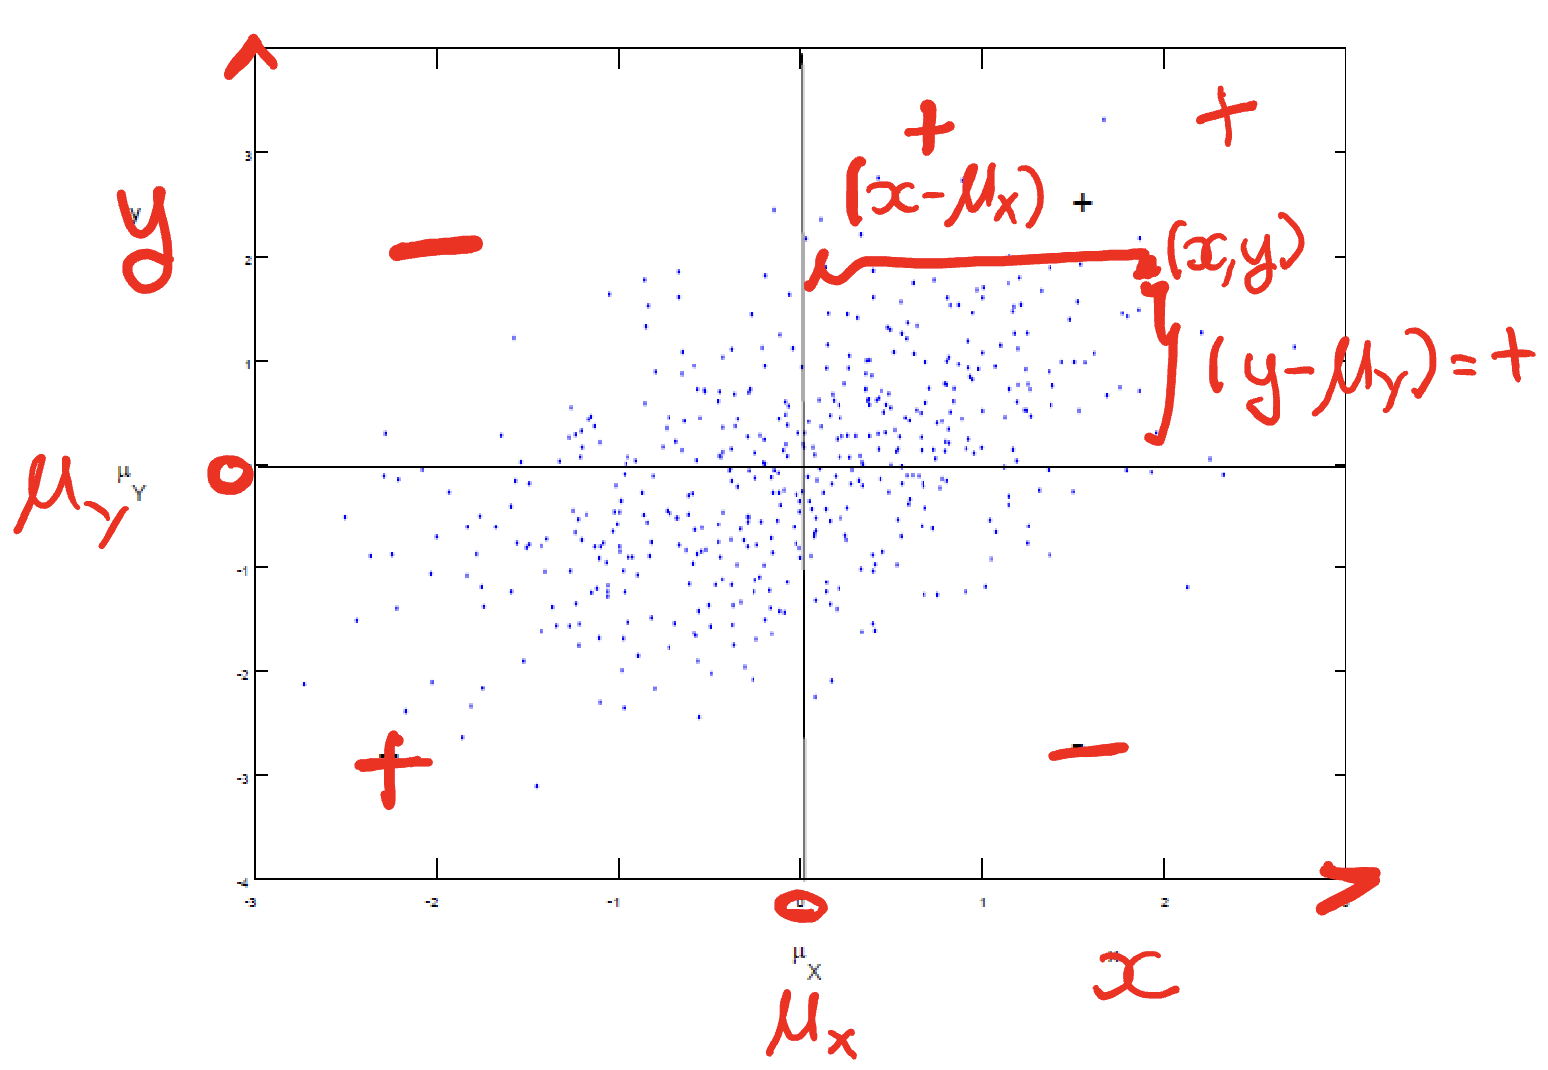
\includegraphics[scale=0.5]{img/cov.png}
    \caption{Random points $(X,Y)$ with covariance 0.5, variances 1.}
\end{figure}


\begin{theorem}
    If $X$ and $Y$ are independent then $\Cov{X, Y} = 0$.
\end{theorem}

\begin{note}
    The converse it NOT true.
\end{note}

% \begin{proof}
%     Recall that $\expect{X - \mu_X} = \expect{X} - \mu_X = 0$. Let $X$ and $Y$ be independent.  \\
%     Then $f(x, y) = f_1(x)f_2(y)$.
%     \begin{align*}
%         \Cov{X, Y} &= \expect{(X - \mu_X)(Y - \mu_Y)}   \\
%                    &= \sum_{\text{all } y} \left[\sum_{\text{all } x} (x - \mu_X)(y - \mu_Y)f_1(x)f_2(y)\right] \\
%                    &= \sum_{\text{all } y} \left[(y - \mu_Y)f_2(y)\sum_{\text{all } x} (x - \mu_X)f_1(x)\right] \\
%                    &= \sum_{\text{all } y} \left[(y - \mu_Y)f_2(y)\expect{X - \mu_X}\right] \\
%                    &= \sum_{\text{all } y} 0    \\
%                    &= 0.
%     \end{align*}
% \end{proof}
% This result can also be proved using the Theorem below.

\begin{theorem}
    Suppose $X$ and $Y$ are independent random variables. Then, if $g_1(X)$ and
    $g_2(Y)$ are two functions, we have
    \[\expect{g_1(X)g_2(Y)} = \expect{g_1(X)}\expect{g_2(Y)}.\]
\end{theorem}

\begin{note}
    $\expect{XY} = \displaystyle \sum_{\text{all $(x,y)$}} xyf(x,y) = \displaystyle \sum_{\text{all $x$}} \displaystyle \sum_{\text{all $y$}} xyf(x,y)$.
\end{note}

\pagebreak

\begin{definition}[\textbf{Correlation Coefficient}]
    The \textbf{correlation coefficient} of $X$ and $Y$ is
    \[\rho = \Corr{X,Y} = \frac{\Cov{X, Y}}{\sigma_X \sigma_Y}.\]    
\end{definition}

\begin{note}
    Alternatively, $\rho = \dis \frac{\Cov{X,Y}}{\sqrt{\Var{X} \Var{Y}}}$.
\end{note}

The correlation coefficient measures the strength of the \textbf{linear} relationship between $X$ and $Y$, it is essentially
a rescaled version of the covariance, scaled to lie in the interval $[-1, 1]$.




\begin{theorem}[\textbf{Properties of $\rho$}]
    \phantom{}\
    \begin{enumerate}
        \item Since $\sigma_X$, $\sigma_Y > 0$, $\rho$ will have the same sign as $\Cov{X,Y}$. Hence the interpretation of the sign of $\rho$ is the same as for $\Cov{X,Y}$, and $\rho = 0$ if $X$ and $Y$ are independent. When $\rho = 0$, we say that $X$ and $Y$ are uncorrelated.
        \item $-1 \leq \rho \leq 1$ and as $\rho \to \pm 1$ the relation between $X$ and $Y$ becomes one-to-one and linear.
    \end{enumerate}
\end{theorem}


\begin{example}
    The joint probability function of $(X,Y)$ is:
    \[
        \begin{array}{cc|ccc|c}
            & & \multicolumn{3}{c|}{x} & \\
            \multicolumn{2}{c|}{f(x,y)} & 0 & 1 & 2 & f_Y(y) \\
            \hline
            \multirow{2}{*}{y} 
              & 1 & 0.06 & 0.15 & 0.09 & 0.3 \\
              & 2 & 0.14 & 0.35 & 0.21 & 0.7 \\
            \hline
            \multicolumn{2}{c|}{f_X(x)} & 0.2 & 0.5 & 0.3 & 1
        \end{array}
    \]
    Calculate the correlation coefficient. What does this say about the relationship between $X$ and $Y$?

    \textbf{Solution:} $\expect{Y} = (1 \times 0.7) = 0.7$, $\expect{X} = (1 \times 0.5) + (2 \times 0.3) = 1.1$, $\expect{XY} = (1 \times 1 \times 0.35) + (2 \times 1 \times 0.21) = 0.77$. 

    $\implies \Cov{X,Y} = 0.77 - (0.7 \times 1.1) = 0$. So $\rho = \Corr{X,Y} = \frac{0}{\sigma_X \sigma_Y} = 0$. \\
    Therefore, $X$ and $Y$ have no linear association (and $X$ and $Y$ are independent).
\end{example}

\subsection{Mean and Variance of a Linear Combination of Random Variables}

\begin{theorem}[\textbf{Results for Expectations}]
    \phantom{}
    \begin{enumerate}
        \item $\expect{aX+bY} = a\expect{X} + b\expect{Y}$.
        \item Let $a_i$ be constants and $\expect{X_i} = \mu_i$, $i = 1,2,\ldots ,n$. Then $\expect{\displaystyle \sum_{i=1}^{n} a_iX_i} = \displaystyle \sum_{i=1}^{n} a_i \mu_i$. In particular, $\expect{\displaystyle \sum_{i=1}^{n} X_i}  = \displaystyle \sum_{i=1}^{n} \expect{X_i}$. \vspace{1mm}
        \item Let $X_1, X_2,\ldots , X_n$ be random variables which have mean $\mu$. Then, the sample mean is $\overline{X} = \dis \frac{\displaystyle \sum_{i=1}^{n} X_i}{n}$ and $\expect{\overline{X}} = \mu$. 
    \end{enumerate}
\end{theorem}

\begin{theorem}[\textbf{Results for Covariance}]
    \phantom{}
    \begin{enumerate}
        \item $\Cov{X,Y} = \Var{X}$.
        \item $\Cov{aX+bY,cU+dV} = ac\Cov{X,U} + ad\Cov{X,V} \\ \hspace*{40mm}+ bc\Cov{Y,U} + bd\Cov{Y,V}$.
    \end{enumerate}
\end{theorem}
\begin{note}
    Covariance is symmetric: $\Cov{X,Y} = \Cov{Y,X}$. And for all $c\in \R$, $\Cov{c,X} = 0$.
\end{note}

\begin{theorem}[\textbf{Results for Variance}]
    \phantom{}
    \begin{enumerate}
        \item \textbf{Variance of a linear comobination:} \vspace{-3mm}
        \[
            \Var{aX+bY} = a^2\Var{X} + b^2\Var{Y} + 2ab\Cov{X,Y}.
        \]
        \item \textbf{Variance of a sum of independent random variables:} \\
        Let $X$ and $Y$ be independent. Since $\Cov{X,Y} = 0$, result 1 gives \vspace{-3mm}
        \[
            \Var{X+Y} = \Var{X} + \Var{Y} = \Var{X-Y}.
        \]
        \item \textbf{Variance of a general linear combination of random variables:} \\
        Let $a_i$ be constants. Then \vspace{-3mm}
        \[
            \Var{\displaystyle \sum_{i=1}^{n} a_iX_i} = \displaystyle \sum_{i=1}^{n} a_i^2\Var{X_i} + 2\displaystyle \sum_{i=1}^{n} \sum_{j=i+1}^{n} a_i a_j \Cov{X_i,X_i}. 
        \]
        \pagebreak
        \item \textbf{Variance of a linear combination of independent random variables:} \\
        Special cases of result 3 are:
        \begin{enumerate}
            \item If $X_1, X_2, \ldots, X_n$ are independent, then $\Cov{X_i,X_j} = 0$, so that \vspace{-3mm}
            \[
                \Var{\displaystyle \sum_{i=1}^{n} a_iX_i} = \displaystyle \sum_{i=1}^{n} a_i^2\Var{X_i}.
            \]
            \item If $X_1, X_2, \ldots, X_n$ are independent and all have the same variance $\Var{X} = \sigma^2$, then \vspace{-3mm}
            \[
                Var{\left( \overline{X} \right)} = \frac{\sigma^2}{n}.
            \]
        \end{enumerate}
    \end{enumerate}
\end{theorem}

\begin{remark}
    If $X_1,X_2,\ldots ,X_n$ are independent random variables with the same mean $\mu$ and the same variance $\sigma^2$, then the sample mean $\overline{X} = \frac{1}{n}\displaystyle \sum_{i=1}^{n} X_i$ has \vspace{-3mm}
    \[
        \expect{\overline{X}} = \mu \quad \text{and} \quad \Var{\overline{X}} = \frac{\sigma^2}{n}.
    \]
    What does this tell us about $\overline{X}$? 
    
    $\implies \overline{X}$ is less variable than $X_i$ (the larger $n$ is the less variability there is).
    \begin{itemize}
        \item This happens because as n increases, e are adding more
        information and so our sample mean. $\overline{X}$ is becoming \textbf{more precise} in sense that we have \vspace{-3mm}
        \[
            \Var{\overline{X}} \to 0 \text{ as } n \to \infty.
        \]
        \item This implies that as $n\to \infty$, $\overline{X} \to \mu$.
        \item This is something called the ``\textbf{law of averages}''.
    \end{itemize}
\end{remark}

\pagebreak


\subsection{Linear Combinations of Independent Normal Random Variables}

\begin{theorem}[\textbf{Linear Combinations of Independent Normal Random Variables}]
    \phantom{}
    \begin{enumerate}
        \item Let $X \sim N(\mu, \sigma^2)$ and $Y = aX + b$, where $a$, $b \in \R$.
        Then, $Y \sim N(a\mu + b, a^2\sigma^2)$.
        \item Let $X \sim N(\mu_1, \sigma_1^2)$ and $Y \sim N(\mu_2, \sigma_2^2)$ be independent random variables, and let $a$ and $b$ be constants.
        Then, $aX+bY \sim \text{N}(a\mu_1 + b\mu_2, a^2\sigma_1^2 + b^2\sigma_2^2)$. \\
        In general, if $X_i \sim \text{N}(\mu_i, \sigma_i^2)$, $i=1,2,\ldots,n$, are independent random variables and $a_1,a_2,\ldots a_n \in \R$, then $\displaystyle \sum_{i=1}^{n} a_iX_i \sim \text{N}\left( \displaystyle \sum_{i=i}^{n} a_i\mu_i, \displaystyle \sum_{i=1}^{n} a_i^2 \sigma_i^2 \right)$.
        \item Let $X_1, X_2, \ldots, X_n$ be independent $N(\mu, \sigma^2)$ random variables. Then
        $\dis \sum_{i=1}^{n} X_i \sim N(n\mu, n\sigma^2)$ and $\overline{X} \sim N(\mu, \frac{\sigma^2}{n})$.
    \end{enumerate}
\end{theorem}

\begin{note}
    We have $\expect{aX+b} = a\mu + b$ and $\Var{aX+b} = a^2\sigma^2$. \\
\end{note}

\begin{example}
    Let $X \sim \text{N}(3,5)$ and $Y \sim \text{N}(6,14)$ be independent random variables. Find $P(X > Y)$.

    \textbf{Solution:} Note that $P(X > Y) = P(X - Y > 0)$. Let $W = X - Y$. Then $\expect{W} = \expect{X} - \expect{Y} = 3 - 6 = -3$ and $\Var{W} = \Var{X} + \Var{Y} = 5 + 14 = 19$ since $X$ and $Y$ are independent. So $W \sim \text{N}(-3,19)$. \vspace{-3mm}
    \begin{align*}
        P(X > Y) & = P(W > 0) \\
        &= P(Z > \frac{0-(-3)}{\sqrt{19}}) \\
        &= P(Z > 0.69) \\
        &= 1 - P(Z \leq 0.69) = 0.245.
    \end{align*}
\end{example}

\begin{example}
    Let $X \sim \text{N}(5,4)$. An independent random variable $Y$ is also normal with mean 7 and standard deviation of 3. Find:
    \begin{enumerate}[label=(\alph*)]
        \item The probability $2X$ differs from $Y$ by more than 4.
        \item The minimum number, $n$, of independent observations needed on $X$ so that $P(|\overline{X} -5| < 0.1) \geq 0.98$.
    \end{enumerate}
    \pagebreak

    \textbf{Solution:}
    \begin{enumerate}[label=(\alph*)]
        \item Let $W = 2X - Y$. Then $\expect{W} = 2\expect{X} - \expect{Y} = 10 - 7 = 3$ and $\Var{W} = 4\Var{X} + \Var{Y} = 16 + 3^2 = 25$. Next, \vspace{-3mm}
        \begin{align*}
            P(|2X - Y|> 4) = P(|W|>4) &= P(W>4) + P(W<4) \\
            &= P(Z > \frac{4-3}{5}) + P(Z < \frac{-4-3}{5}) \\
            &= P(Z > 0.2) + P(Z < -1.4) \\
            &= \left[ 1 - P(Z \leq 0.2) \right] + \left[ 1 - P(Z \leq 1.4) \right]
        \end{align*}
        \item We have that $\overline{X} \sim \text{N}(\mu = 5, \frac{\sigma^2}{n} = \frac{4}{n})$. 
        \begin{align*}
            P(|\overline{X} -5| < 0.1) &\geq 0.98 \\
            P(-0.1 < \overline{X} - 5 < 0.1) &\geq 0.98 \\
            P(\frac{-0.1}{\sqrt{\frac{4}{n}}} < Z < \frac{0.1}{\sqrt{\frac{4}{n}}}) &\geq 0.98 \\
            \implies P(Z \leq \frac{0.1}{\sqrt{\frac{4}{n}}}) &\geq 0.99 \quad \text{use a graph...} \\
            \frac{0.1}{\sqrt{\frac{4}{n}}} &\geq 2.33 \implies n \geq 2171.56 \\
            n &= 2172.
        \end{align*}
        More precisely, use R to get $n \geq 2165$.
    \end{enumerate}
\end{example}


\pagebreak

\subsection{Indicator Random Variables}

An indicator variable is a binary variable (0 or 1) that indicates whether or not an event has occurred. It can allow us to take more complicated scenarios and break them into simpler ones.

\begin{example}
    Let $X \sim \text{N}(n,p)$. Define new random variables $X_i$ by \vspace{-3mm}
    \[
        X_i = 
        \begin{cases} 
            0 & \text{if $i^{\text{th}}$ trial was a failure} \\
            1 & \text{if $i^{\text{th}}$ trial was a success}
        \end{cases}.
    \]

    The random variable $X_i$ indicates whether `success' occured on the $i^\text{th}$ trial. The total number of successes is $X = \displaystyle \sum_{i=1}^{n} X_i$. We can find the mean and variance of $X_i$ and then use our results for mean and variance to find $\mu$ and $\sigma^2$ of $X$. First, \vspace{-3mm}
    \[
        \expect{X_i} = \displaystyle \sum_{x_1=0}^{1} f(x_i) = 0f(0) + 1f(1) = f(1). 
    \]
    But $f(1) = p$ since $P(\text{success}) = p$ on each trial. Therefore $\expect{X_i} = p$. And since $X_i = 0$ or 1, so $X_i = X_i^2$, and therefore 
    \[
        \expect{X_i^2} = \expect{X_i} = p.
    \]
    Thus, 
    \[
        \Var{X_i} = \expect{X_i^2} - \left( \expect{X_i} \right)^2 = p - p^2 = p(1-p).
    \]
    In the Binomial distribution the trials are independent, so the $X_i$'s are also independent. Thus
    \begin{align*}
        \expect{X} &= \expect{\displaystyle \sum_{i=1}^{n} X_i} = \displaystyle \sum_{i=1}^{n} \expect{X_i} = \displaystyle \sum_{i=1}^{n} p = np. \\
        \Var{X} &= \Var{\displaystyle \sum_{i=1}^{n} X_i} = \displaystyle \sum_{i=1}^{n} \Var{X_i} = \displaystyle \sum_{i=1}^{n} p(1-p) = np(1-p).
    \end{align*}
\end{example}

\begin{remark}
    Note that $X_i \sim \text{Binomial}(1,p)$ is actually a Binomial random variable. In some problems the $X_i$'s are not independent, we will also need covariances.
\end{remark}


\pagebreak

\begin{example}
    We have $N$ letters to $N$ different people, and $N$ envelopes addressed to those $N$ people. One letter is put in each envelope at random. Find the mean and variance of the number of letters placed in the right envelopes.

    \textbf{Solution:}
    Let
    \[
        X_i = 
        \begin{cases} 
            0 & \text{if letter $i$ is not in envelope $i$} \\
            1 & \text{if letter $i$ is in envelope $i$}
        \end{cases}.
    \]

    Then, the total number of correctly placed letters is $\displaystyle \sum_{i=1}^{N} X_i$. Note that $X_i$'s are dependent since the experiment is done without replacenent!
    \[
        \expect{X_i} = \displaystyle \sum_{x_i=0}^{1} x_if(x_i) = f(1) = \frac{1}{N} = \expect{X_i^2}
    \]
    since there is 1 chance in $N$ that letter $i$ will be put in envelope $i$ and then,
    \[
        \Var{X_i} = \expect{X_i} - \left( \expect{X_i} \right)^2 = \frac{1}{N} - \frac{1}{N^2} = \frac{1}{N}\left( 1 - \frac{1}{N} \right).
    \]
    Therefore,
    \[
        \expect{\displaystyle \sum_{i=1}^{N} X_i} = \displaystyle \sum_{i=1}^{N} \expect{X_i} = \displaystyle \sum_{i=1}^{N} \frac{1}{N} = 1.
    \]
    To find $\Var{\displaystyle \sum_{i=1}^{N} X_i}$, we need to calculate the covariance terms since $X_i$'s are dependent. \\
    Next, $\Cov{X_i,X_j} = \expect{X_i X_j} - \expect{X_i} \expect{X_j}$ for $i \neq j$. So, we need
    \[
        \expect{X_i X_j} = \displaystyle \sum_{x_i = 0}^{1} \displaystyle \sum_{x_j=0}^{1} x_i x_j f(x_i,x_j) = f(1,1) = P(X_i = 1, X_j = 1) = P(A \cap B).
    \]
    where $A = \text{letter $i$ is placed in envelop $i$}$, $B = \text{letter $j$ is placed in envelop $j$}$.
\end{example}





\newpage